\chapter{Testing and launching}
\label{testing}

This chapter presents the snapshots from launching of the application and short description of testing methods and processes. 

\section{Examples of launching}
The game can be launched in two modes - normal and debug. Normal presents enough functionality for children to play it, while debug mode offers additional functionalities for therapist and/or developer. 
\subsection{Normal mode}
\begin{figure} [h]
\begin{center}
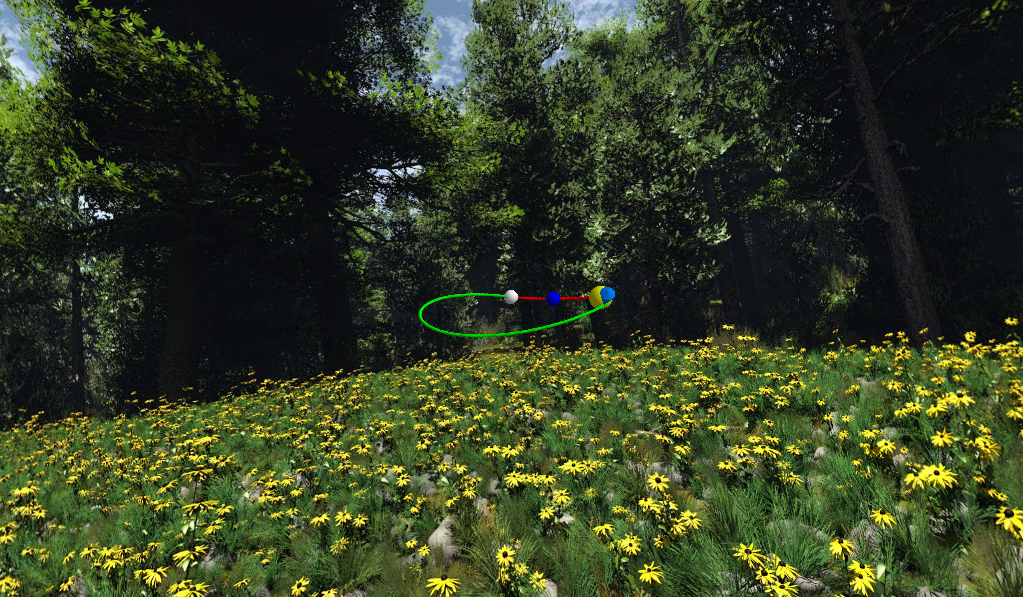
\includegraphics[width=0.7\textwidth]{Images/first_curve}
\end{center}
\caption{First curve (Lowest level).}
\label{fig:first_curve}
\end{figure}

\begin{figure}
\begin{center}
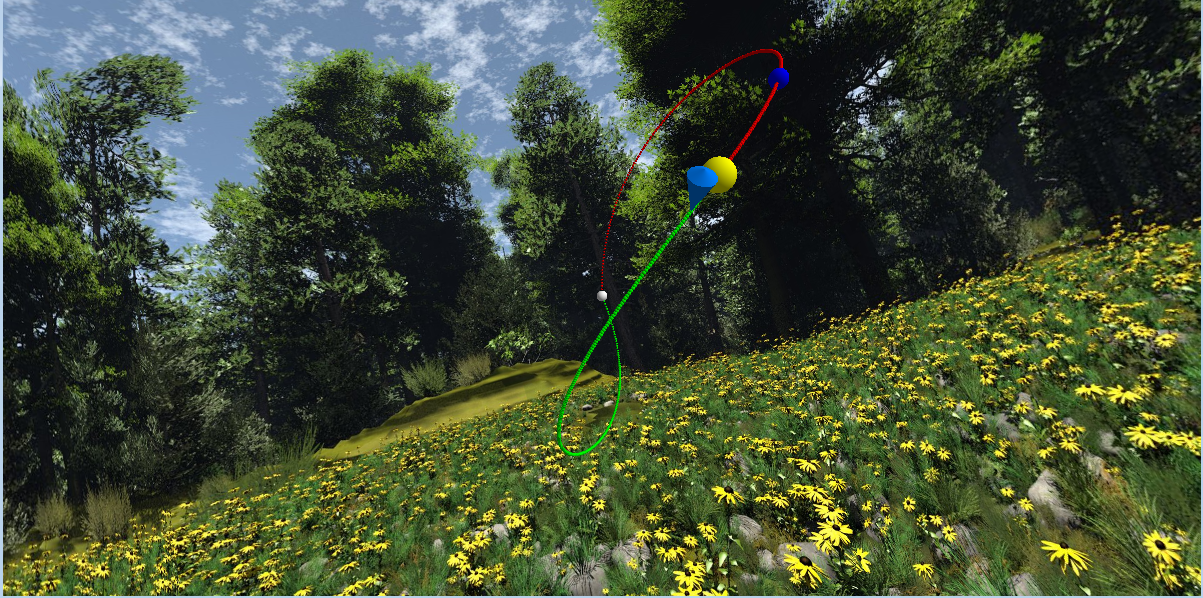
\includegraphics[width=0.7\textwidth]{Images/second_curve}%
\end{center}
\caption{Second curve (Middle level).}
\label{fig:second_curve}
\end{figure}

\begin{figure}
\begin{center}
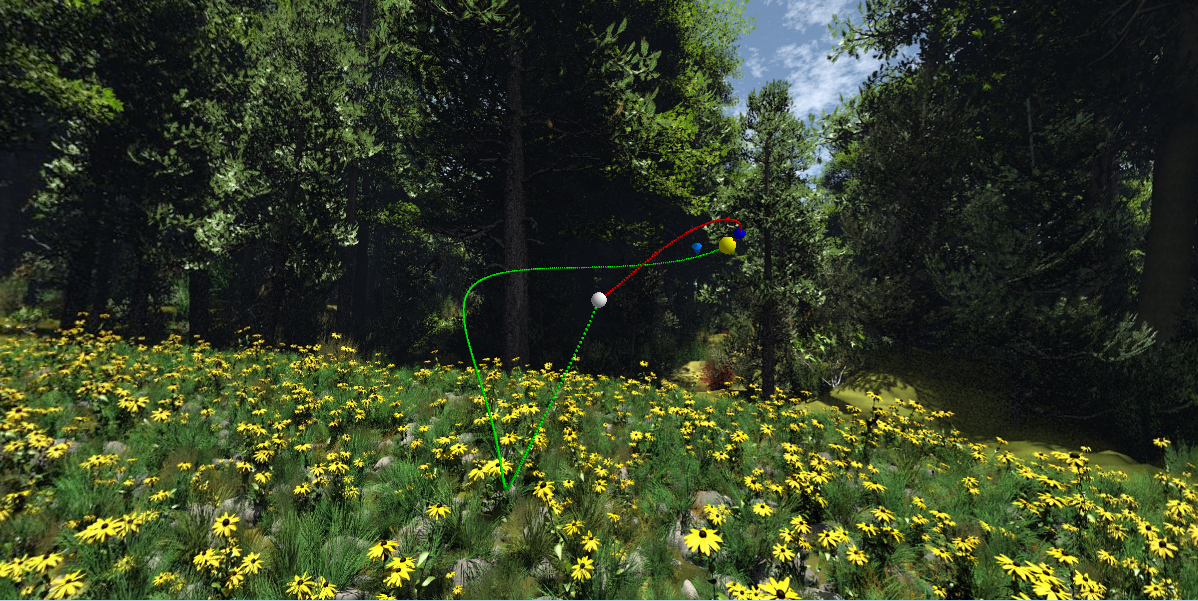
\includegraphics[width=0.7\textwidth]{Images/third_curve}%
\end{center}
\caption{Third curve (Highest level).}
\label{fig:third_curve}
\end{figure}

\begin{figure}
\begin{center}
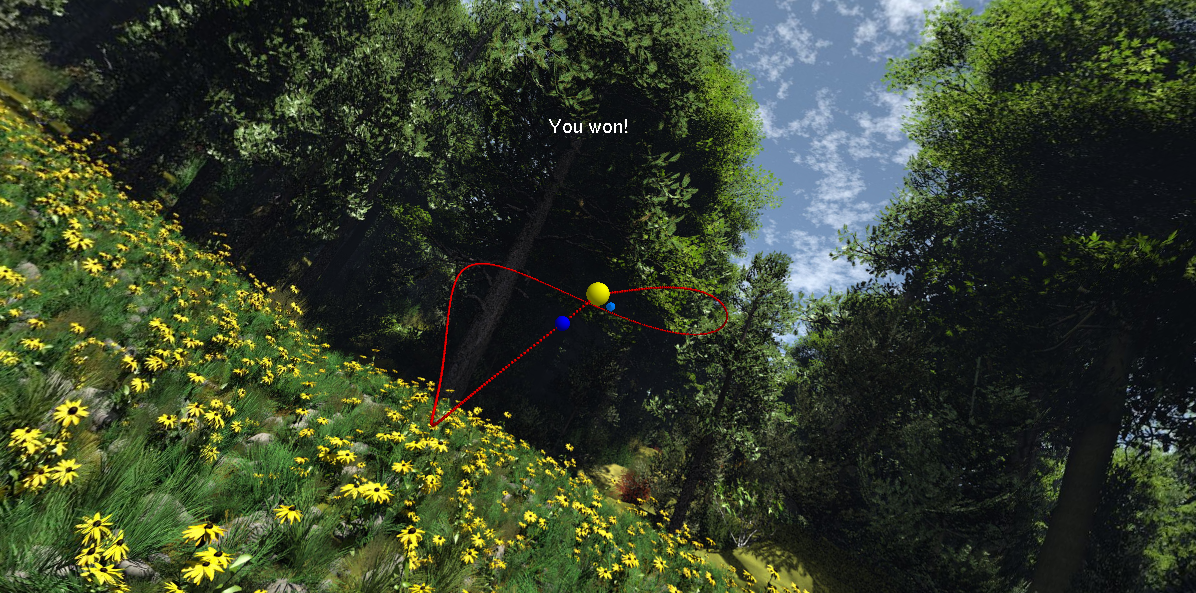
\includegraphics[width=0.7\textwidth]{Images/won}%
\end{center}
\caption{The game is displaying an information about the win.}
\label{fig:win}
\end{figure}

In the figures \emph{\ref{fig:first_curve}, \ref{fig:second_curve}, \ref{fig:third_curve}} three paths from game are presented. White sphere is a start/end point. Blue sphere is the competitor's object. Yellow sphere is the player's object and the cursor is presented as a blue cone. The passed distance is marked with green color. The message about winning and state of the game just after level restart is presented in the figure \emph{\ref{fig:win}} 

\subsection{Debug mode}
Figures \emph{\ref{fig:no_skybox}, \ref{fig:route}, \ref{fig:points}} present different toggled debug option. In figure \emph{\ref{fig:route}} the player's object real route is showed. The sharp impulses are effects of sudden getting out of the range of magnetic attraction field (it requires pressure which is hard to control when the field disappears).
\begin{figure}
\begin{center}
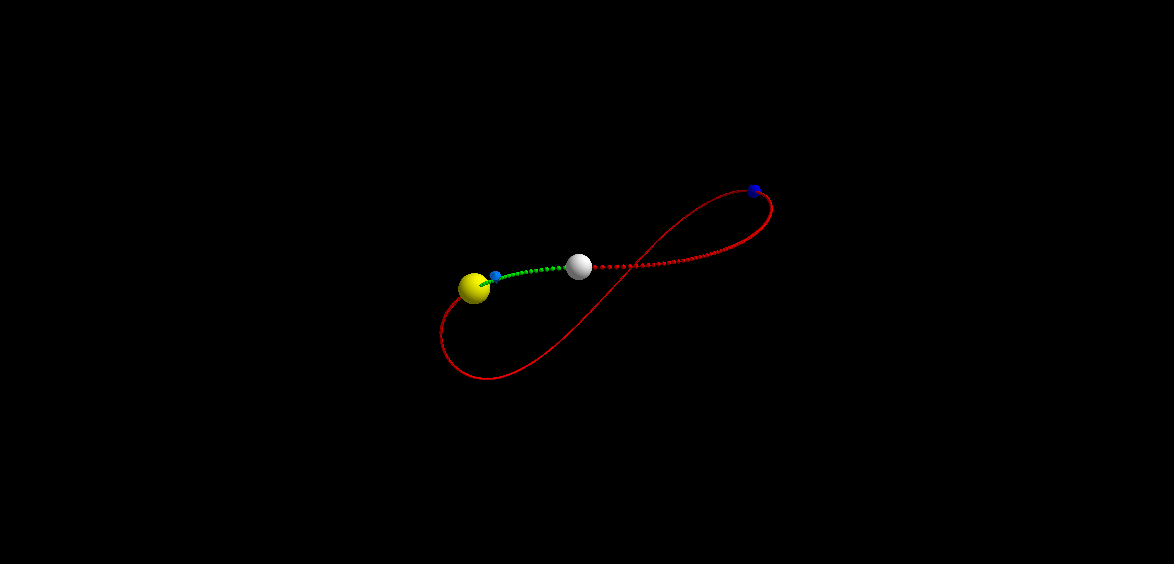
\includegraphics[width=0.7\textwidth]{Images/noskybox}%
\end{center}
\caption{Scene view without the skybox.}
\label{fig:no_skybox}
\end{figure}

\begin{figure}
\begin{center}
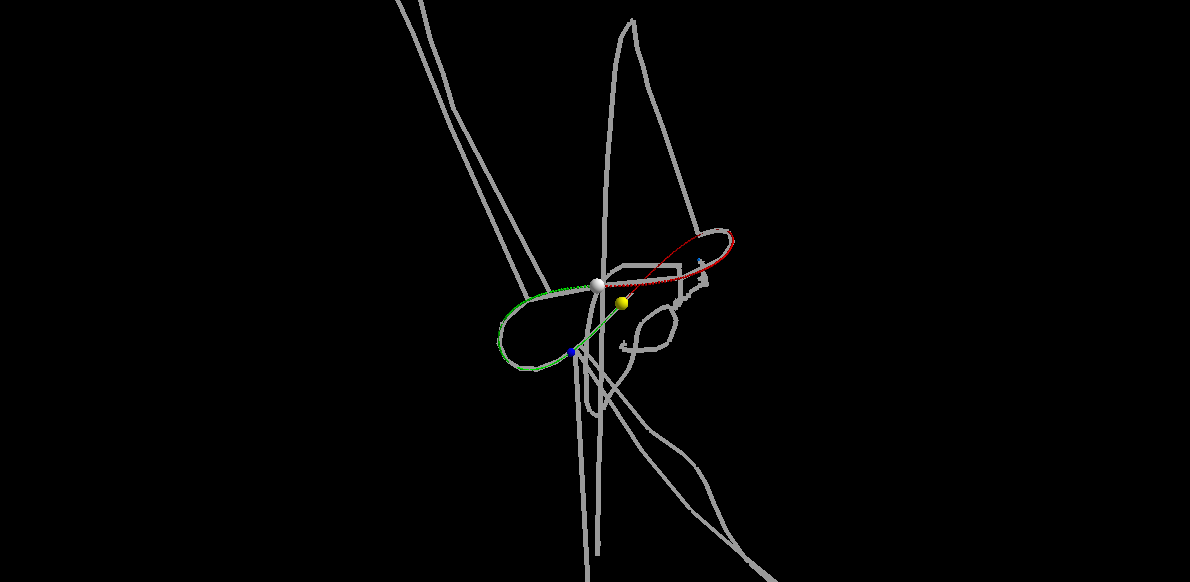
\includegraphics[width=0.7\textwidth]{Images/route}%
\end{center}
\caption{The route of the player's object.}
\label{fig:route}
\end{figure}

\begin{figure}
\begin{center}
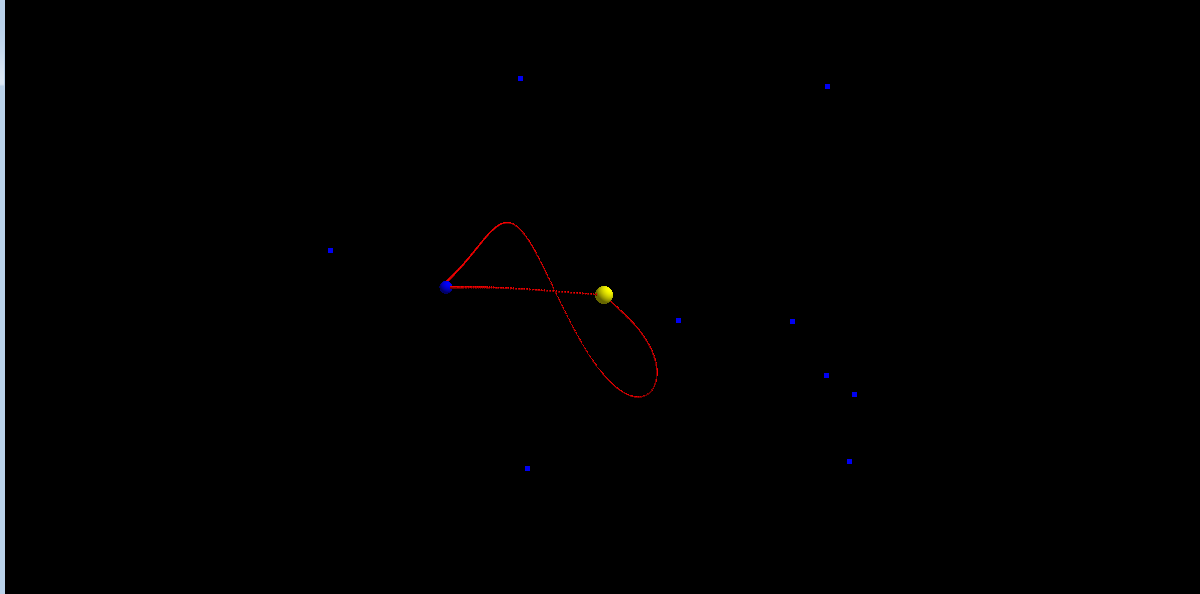
\includegraphics[width=0.7\textwidth]{Images/points}%
\end{center}
\caption{Control points of presented Bezier's curve.}
\label{fig:points}
\end{figure}

\section{Testing}
Because developed application is a game, testing was focused on specification-based testing(requirements based on analysis and design phase) and visual testing. There was a small number of unit tests on first stage of development in order to check mathematical function correctness. 
The following subsections present screen-shots and descriptions of specification-based tests. Presented requirements are based on \emph{\ref{design} : \nameref{design}}.

\subsection{Haptic thread}
Testing of haptic thread is presented on the film attached on CD's. The following statements were tested positively:
\begin{itemize} [noitemsep]
\item "Cursor should get attracted by path and be able to push the Bait."
\item "Cursor should be able to get off the path."
\item "The path should be smooth in touch and consistent with graphic representation."

It is very important requirement, because display path and haptic path are two different shapes, as described in \emph{\ref{path_representation} : \nameref{path_representation}}. 
\end{itemize}
\subsection{Game logic}
Majority of the game logic is connected with levelling mechanism. The rest regards the problems of display and resetting and setting new objects properties before new round.
\begin{itemize} [noitemsep]
\item "The player should level up when he moves the project from start to end in time equal or less than specified for this curve and competitor winning time."

This requirement's testing can albo be seen on the film.
\item "The message should show up when player advance to the next level."

This requirement was tested positively in \emph{\ref{fig:win} : \nameref{fig:win}}.

\item "The Bait and Racer should start new round from start point"

This requirement was tested positively in \emph{\ref{fig:win} : \nameref{fig:win}}.
\end{itemize}


